\documentclass[tikz,border=9pt]{standalone}
\usepackage{amsmath}
\usetikzlibrary{arrows.meta}
\definecolor{newframe}{RGB}{30,100,175}
\definecolor{spin}{RGB}{190,65,30}
\begin{document}
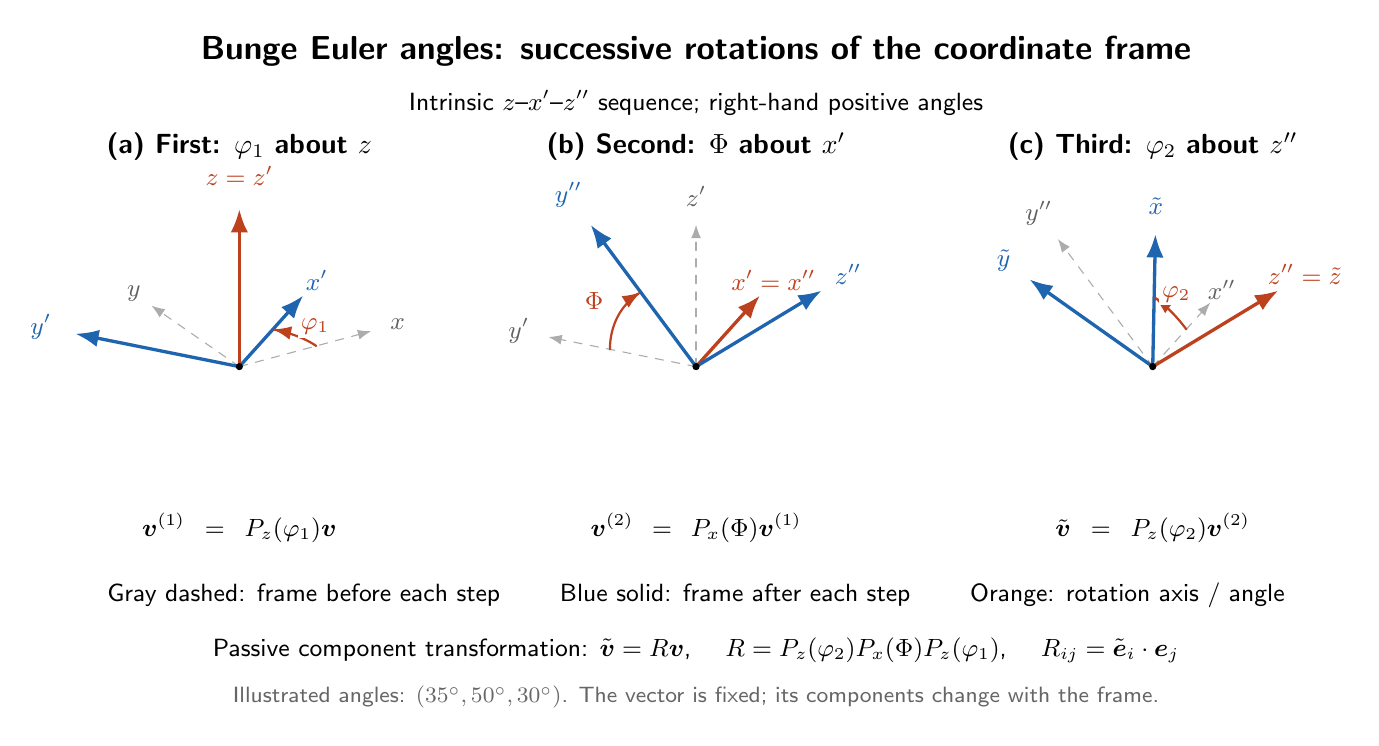
\begin{tikzpicture}[>=Latex,font=\sffamily\small,line cap=round,line join=round]
\node[font=\sffamily\bfseries\large] at (5.8,4.0) {Bunge Euler angles: successive rotations of the coordinate frame};
\node[align=center] at (5.8,3.35) {Intrinsic $z$--$x^{\prime}$--$z^{\prime\prime}$ sequence; right-hand positive angles};
\begin{scope}[shift={(0.0,0)}]
\node[font=\sffamily\bfseries] at (0,2.8) {(a) First: $\varphi_1$ about $z$};
\draw[->,gray!65,dashed] (0,0)--(1.67400,0.45000);
\node[gray!75!black,fill=white,inner sep=1pt] at (2.00880,0.54000) {$x$};
\draw[->,gray!65,dashed] (0,0)--(-1.11600,0.77400);
\node[gray!75!black,fill=white,inner sep=1pt] at (-1.33920,0.92880) {$y$};
\draw[->,newframe,very thick] (0,0)--(0.81239,0.90285);
\node[newframe,fill=white,inner sep=1pt] at (0.98299,1.09245) {$x^{\prime}$};
\draw[->,newframe,very thick] (0,0)--(-2.08260,0.41768);
\node[newframe,fill=white,inner sep=1pt] at (-2.51995,0.50540) {$y^{\prime}$};
\draw[->,spin,very thick] (0,0)--(0.00000,2.00000);
\node[spin,fill=white,inner sep=1pt] at (0.00000,2.42000) {$z=z^{\prime}$};
\draw[->,spin,thick] (0.97650,0.26250)--(0.96465,0.27057)--(0.95248,0.27855)--(0.94001,0.28644)--(0.92723,0.29424)--(0.91416,0.30195)--(0.90079,0.30955)--(0.88713,0.31706)--(0.87318,0.32447)--(0.85895,0.33177)--(0.84445,0.33896)--(0.82967,0.34604)--(0.81462,0.35301)--(0.79931,0.35987)--(0.78374,0.36661)--(0.76792,0.37324)--(0.75186,0.37974)--(0.73555,0.38612)--(0.71900,0.39237)--(0.70222,0.39850)--(0.68521,0.40450)--(0.66798,0.41037)--(0.65054,0.41611)--(0.63288,0.42171)--(0.61502,0.42718)--(0.59697,0.43251)--(0.57872,0.43770)--(0.56028,0.44275)--(0.54166,0.44765)--(0.52287,0.45241)--(0.50391,0.45703)--(0.48479,0.46150)--(0.46551,0.46581)--(0.44608,0.46998)--(0.42650,0.47400);
\node[spin,fill=white,inner sep=1pt] at (0.95971,0.50379) {$\varphi_1$};
\fill (0,0) circle (1.3pt);
\node[align=center,text width=4.8cm] at (0,-2.05) {$\boldsymbol v^{(1)}=P_z(\varphi_1)\boldsymbol v$};
\end{scope}
\begin{scope}[shift={(5.8,0)}]
\node[font=\sffamily\bfseries] at (0,2.8) {(b) Second: $\Phi$ about $x^{\prime}$};
\draw[->,gray!65,dashed] (0,0)--(-1.87434,0.37591);
\node[gray!75!black,fill=white,inner sep=1pt] at (-2.24921,0.45110) {$y^{\prime}$};
\draw[->,gray!65,dashed] (0,0)--(0.00000,1.80000);
\node[gray!75!black,fill=white,inner sep=1pt] at (0.00000,2.16000) {$z^{\prime}$};
\draw[->,spin,very thick] (0,0)--(0.81239,0.90285);
\node[spin,fill=white,inner sep=1pt] at (0.98299,1.09245) {$x^{\prime}=x^{\prime\prime}$};
\draw[->,newframe,very thick] (0,0)--(-1.33867,1.80057);
\node[newframe,fill=white,inner sep=1pt] at (-1.61979,2.17869) {$y^{\prime\prime}$};
\draw[->,newframe,very thick] (0,0)--(1.59536,0.96561);
\node[newframe,fill=white,inner sep=1pt] at (1.93039,1.16839) {$z^{\prime\prime}$};
\draw[->,spin,thick] (-1.09337,0.21928)--(-1.09301,0.24616)--(-1.09193,0.27287)--(-1.09013,0.29940)--(-1.08761,0.32574)--(-1.08437,0.35186)--(-1.08043,0.37775)--(-1.07577,0.40339)--(-1.07040,0.42876)--(-1.06432,0.45386)--(-1.05755,0.47865)--(-1.05008,0.50313)--(-1.04191,0.52727)--(-1.03306,0.55107)--(-1.02353,0.57451)--(-1.01333,0.59757)--(-1.00246,0.62023)--(-0.99093,0.64249)--(-0.97874,0.66432)--(-0.96591,0.68571)--(-0.95244,0.70666)--(-0.93835,0.72713)--(-0.92364,0.74713)--(-0.90832,0.76664)--(-0.89240,0.78564)--(-0.87590,0.80412)--(-0.85881,0.82208)--(-0.84116,0.83949)--(-0.82296,0.85635)--(-0.80421,0.87265)--(-0.78494,0.88837)--(-0.76515,0.90350)--(-0.74485,0.91804)--(-0.72407,0.93198)--(-0.70280,0.94530);
\node[spin,fill=white,inner sep=1pt] at (-1.29292,0.83829) {$\Phi$};
\fill (0,0) circle (1.3pt);
\node[align=center,text width=4.8cm] at (0,-2.05) {$\boldsymbol v^{(2)}=P_x(\Phi)\boldsymbol v^{(1)}$};
\end{scope}
\begin{scope}[shift={(11.6,0)}]
\node[font=\sffamily\bfseries] at (0,2.8) {(c) Third: $\varphi_2$ about $z^{\prime\prime}$};
\draw[->,gray!65,dashed] (0,0)--(0.73115,0.81257);
\node[gray!75!black,fill=white,inner sep=1pt] at (0.87738,0.97508) {$x^{\prime\prime}$};
\draw[->,gray!65,dashed] (0,0)--(-1.20480,1.62051);
\node[gray!75!black,fill=white,inner sep=1pt] at (-1.44576,1.94462) {$y^{\prime\prime}$};
\draw[->,newframe,very thick] (0,0)--(0.03421,1.68218);
\node[newframe,fill=white,inner sep=1pt] at (0.04140,2.03543) {$\tilde x$};
\draw[->,newframe,very thick] (0,0)--(-1.56552,1.10791);
\node[newframe,fill=white,inner sep=1pt] at (-1.89427,1.34058) {$\tilde y$};
\draw[->,spin,very thick] (0,0)--(1.59536,0.96561);
\node[spin,fill=white,inner sep=1pt] at (1.93039,1.16839) {$z^{\prime\prime}=\tilde z$};
\draw[->,spin,thick] (0.42650,0.47400)--(0.41563,0.48850)--(0.40466,0.50288)--(0.39359,0.51715)--(0.38243,0.53129)--(0.37118,0.54531)--(0.35984,0.55920)--(0.34841,0.57295)--(0.33690,0.58657)--(0.32532,0.60005)--(0.31365,0.61339)--(0.30191,0.62658)--(0.29010,0.63962)--(0.27822,0.65252)--(0.26628,0.66525)--(0.25427,0.67783)--(0.24220,0.69025)--(0.23007,0.70251)--(0.21789,0.71460)--(0.20566,0.72652)--(0.19338,0.73826)--(0.18105,0.74983)--(0.16868,0.76123)--(0.15627,0.77244)--(0.14382,0.78347)--(0.13134,0.79431)--(0.11883,0.80497)--(0.10629,0.81544)--(0.09372,0.82571)--(0.08113,0.83578)--(0.06852,0.84566)--(0.05590,0.85534)--(0.04326,0.86481)--(0.03062,0.87408)--(0.01796,0.88314);
\node[spin,fill=white,inner sep=1pt] at (0.30019,0.91661) {$\varphi_2$};
\fill (0,0) circle (1.3pt);
\node[align=center,text width=4.8cm] at (0,-2.05) {$\tilde{\boldsymbol v}=P_z(\varphi_2)\boldsymbol v^{(2)}$};
\end{scope}
\node[align=center] at (5.8,-2.9) {Gray dashed: frame before each step \qquad Blue solid: frame after each step \qquad Orange: rotation axis / angle};
\node[align=center] at (5.8,-3.6) {Passive component transformation: $\tilde{\boldsymbol v}=R\boldsymbol v$, \quad $R=P_z(\varphi_2)P_x(\Phi)P_z(\varphi_1)$, \quad $R_{ij}=\tilde{\boldsymbol e}_i\cdot\boldsymbol e_j$};
\node[font=\sffamily\footnotesize,text=gray!80!black] at (5.8,-4.2) {Illustrated angles: $(35^\circ,50^\circ,30^\circ)$. The vector is fixed; its components change with the frame.};
\end{tikzpicture}
\end{document}
